\documentclass[lettersize,journal]{IEEEtran}
\usepackage{amsmath,amsfonts}
\usepackage{algorithmic}
\usepackage{algorithm}
\usepackage{array}
\usepackage[caption=false,font=normalsize,labelfont=sf,textfont=sf]{subfig}
\usepackage{textcomp}
\usepackage{stfloats}
\usepackage{url}
\usepackage{verbatim}
\usepackage{graphicx}
\usepackage{cite}
\hyphenation{op-tical net-works semi-conduc-tor IEEE-Xplore}
% updated with editorial comments 8/9/2021

% Marker for details only the authors can supply (names, roll numbers, ...).
% Search for "TODO" before submission.
\newcommand{\todo}[1]{\textbf{[TODO: #1]}}

\begin{document}

\title{Reproducing DFF-Adapter: Fine-Grained DINOv2 Tuning with Dual Supervision for Face Forgery Detection and Its Cross-Dataset Generalization}

\author{Author1-RollNo., Author2-RollNo. \todo{replace with names and roll numbers}}

\maketitle

\begin{abstract}
Deepfake detectors that score highly on their training benchmark often fail on unseen manipulations. We reproduce DFF-Adapter~\cite{zhang2026dff}, a parameter-efficient detector that inserts lightweight multi-head LoRA adapters into every transformer block of a frozen DINOv2 backbone and jointly optimises authenticity detection and forgery-type classification through a shared branch. Because of compute limits, we use DINOv2-Small and DINOv2-Base instead of the paper's DINOv2-Large. Trained on FaceForensics++ (c23), our best configuration (Small, 30 epochs) reaches 99.08\% FF++ validation video AUC (paper: 99.56\%) and 82.98\%, 86.25\% and 88.03\% video AUC on Celeb-DF-v1, Celeb-DF-v2 and a 392-video DFDC subset (paper: 96.14\%, 95.26\% and not reported). In-domain performance is thus reproduced to within 0.5 percentage points (pp), while a 9--13~pp gap remains on Celeb-DF. A larger backbone did not improve cross-dataset results: Base trails Small by 4.03~pp video AUC on DFDC. As an extension, we apply label smoothing (0.1) to the forgery-type loss; it did not improve video-level AUC on any of the three unseen sets. All results are single-seed, use different checkpoints for different datasets, and should be read with the caveats listed in Section~\ref{sec:lim}.
\end{abstract}

\begin{IEEEkeywords}
Deepfake detection, DINOv2, LoRA, parameter-efficient fine-tuning, cross-dataset generalization, label smoothing.
\end{IEEEkeywords}

\section{Introduction}
Synthetic face manipulation has become cheap and convincing enough to threaten information integrity, and detection is now a standard stress test for the generalization ability of deep models~\cite{lecun2015deep}. The core difficulty is not accuracy on a known benchmark, which modern detectors saturate, but robustness when the manipulation method, compression, or identity distribution changes.

Recent work therefore adapts large pre-trained vision models. DFF-Adapter~\cite{zhang2026dff} observes that existing DINOv2-based detectors treat the task as generic real/fake classification and typically insert adapters only into the last block or fine-tune only the last few layers. It instead injects low-rank adapters into \emph{every} transformer block and adds an auxiliary forgery-type classification task, so that the authenticity decision can inherit manipulation-specific cues. With only 3.5M trainable parameters, it reports accuracy comparable to or better than much heavier detectors.

\textbf{Project criterion.} We follow the ``reproduce paper results'' criterion: we re-implemented the method from the paper's description and did not run the authors' implementation, so the paper's numbers below are reference values rather than results from our environment. \todo{confirm the criterion and whether the authors' code is public}

\textbf{Contributions.}
\begin{itemize}
\item A re-implementation of DFF-Adapter on frozen DINOv2-Small and DINOv2-Base, trained on FF++ c23 and evaluated on Celeb-DF-v1, Celeb-DF-v2 and a DFDC subset.
\item A side-by-side comparison with the paper's reported video-level AUC and EER, with the size and source of every gap stated explicitly.
\item Controlled comparisons of backbone size and training length, and one extension: label smoothing on the auxiliary forgery-type loss.
\item An explicit list of protocol and checkpoint differences that limit what can be concluded.
\end{itemize}

\textbf{Team composition.}
\begin{itemize}
\item Member 1: \todo{name, roll no., e-mail, contribution}
\item Member 2: \todo{name, roll no., e-mail, contribution}
\end{itemize}

\section{Related Work}
\textbf{Classical forgery detectors.} Early detectors target visible or physical artifacts and later learned blending boundaries and synthetic-forgery cues, e.g., Face X-ray~\cite{li2020facexray} and self-blended images~\cite{shiohara2022sbi}, to improve generalization to unseen manipulations. Their quality is measured on benchmark suites such as FaceForensics++~\cite{rossler2019faceforensics}, Celeb-DF~\cite{li2020celebdf} and DFDC~\cite{dolhansky2020dfdc}.

\textbf{Pre-trained large models.} Vision transformers~\cite{vaswani2017attention,dosovitskiy2021vit} pre-trained at scale provide semantically rich features. DINOv2~\cite{oquab2024dinov2} is a self-supervised backbone with strong transfer, and register tokens~\cite{darcet2024registers} further clean its feature maps; the DFF-Adapter paper uses the registers variant of DINOv2-Large.

\textbf{Parameter-efficient tuning.} LoRA~\cite{hu2022lora} learns low-rank updates to frozen weights, keeping the number of trainable parameters small and preserving pre-training priors.

\textbf{DFF-Adapter.} DFF-Adapter~\cite{zhang2026dff} combines these ideas: low-rank adapters in every transformer block, three branches (authenticity, forgery type, shared), and dual supervision. The authors report the best overall results across five deepfake benchmarks, including cross-dataset and cross-manipulation settings.

\textbf{Label smoothing.} Label smoothing~\cite{szegedy2016rethinking} softens one-hot targets and is often reported to improve calibration and generalization~\cite{muller2019labelsmoothing}. The paper uses hard forgery-type labels; testing smoothed type labels is our extension.

\section{Proposed Methodology}
\subsection{Overview}
Fig.~\ref{fig:pipeline} shows the pipeline. Face crops from a video are encoded by a frozen DINOv2 backbone. A DFF-Adapter in each transformer block feeds three branches: an authenticity branch, a forgery-type branch and a shared branch. During training both tasks are supervised; at inference only the fused authenticity and shared branches are used, so the forgery-type head adds no test-time cost~\cite{zhang2026dff}. The paper also describes a Forgery-Aware Multi-Head Router (FAMHR) and Shared-Enhanced Task Fusion (SETF) inside the adapter. \todo{one or two sentences on how our code implements the multi-head LoRA, FAMHR and SETF, plus LoRA rank}

\begin{figure*}[!t]
\centering
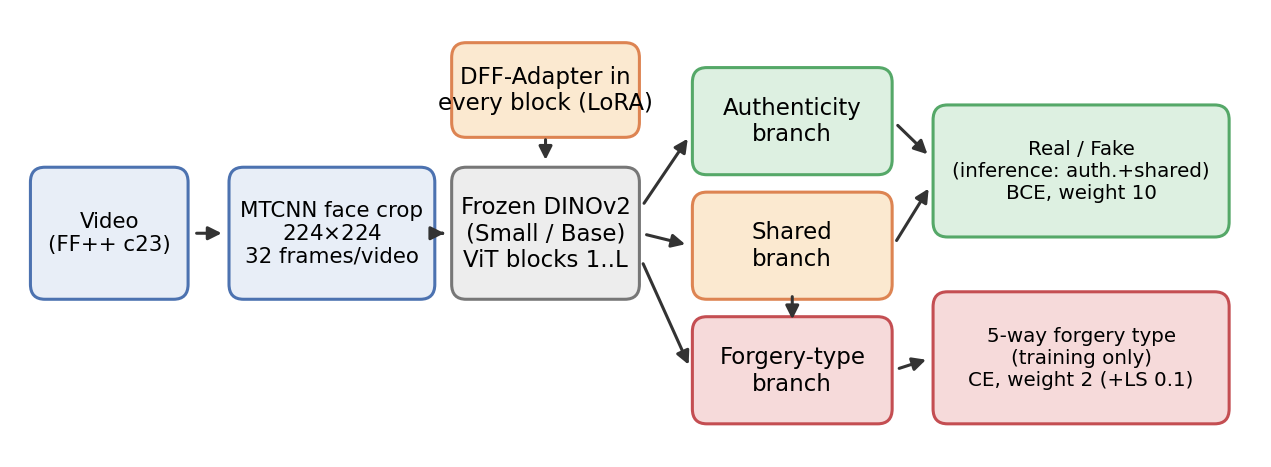
\includegraphics[width=0.86\textwidth]{fig_pipeline}
\caption{Pipeline of our reproduction. Only the adapter parameters are trained; the DINOv2 backbone is frozen. Weights 10 and 2 are the loss weights used in our runs.}
\label{fig:pipeline}
\end{figure*}

\subsection{Backbone and trainable parameters}
We use frozen DINOv2-Small and DINOv2-Base; the paper uses DINOv2-Large. With the Small backbone our model has 667{,}374 trainable parameters, compared with 3.5M reported by the paper for Large.

\subsection{Dual-supervision objective}
Let $y_a\in\{0,1\}$ be the authenticity label and $y_t\in\{1,\dots,K\}$ the forgery type, with $K=5$ classes (original, Deepfakes, Face2Face, FaceSwap, NeuralTextures). With authenticity logit $s$ and type logits $\mathbf{z}$, the loss is
\begin{equation}
\mathcal{L}=\lambda_a\,\mathrm{BCE}\big(s,y_a\big)+\lambda_t\,\mathrm{CE}\big(\mathbf{z},\tilde{\mathbf{y}}_t\big),
\label{eq:loss}
\end{equation}
with $\lambda_a=10$ and $\lambda_t=2$ in all our runs. For the baseline, $\tilde{\mathbf{y}}_t$ is the one-hot vector of $y_t$.

\subsection{Extension: label-smoothed forgery-type supervision}
For the extension, the type target becomes
\begin{equation}
\tilde{\mathbf{y}}_t=(1-\epsilon)\,\mathbf{e}_{y_t}+\frac{\epsilon}{K}\mathbf{1},\qquad \epsilon=0.1,
\label{eq:ls}
\end{equation}
applied \emph{only} to the forgery-type loss; the authenticity BCE is unchanged. The motivation is that manipulation types share artifacts, so hard labels may over-penalise plausible confusions between them.

\subsection{Video-level scoring}
Frame-level authenticity scores of a video are aggregated into one video score, on which video-level AUC and EER are computed. \todo{state the aggregation rule, e.g. mean of frame probabilities}

\section{Experimental Setup}
\subsection{Data}
\textbf{Training and validation.} FaceForensics++ (c23)~\cite{rossler2019faceforensics}: 5{,}000 videos spanning the original class and four manipulations (Deepfakes, Face2Face, FaceSwap, NeuralTextures). Faces are cropped with MTCNN~\cite{zhang2016mtcnn} to $224\times224$ and 32 frames per video are stored. Training samples 10 random frames per video per epoch; validation uses 8 frames per video. \todo{train/val video counts from ffpp\_manifest\_split.csv}

\textbf{Unseen evaluation sets (all crops used).}
\begin{table}[!t]
\caption{Evaluation sets\label{tab:data}}
\centering
\footnotesize
\begin{tabular}{|l||c|c|c|}
\hline
Dataset & Videos & Frames & Note\\
\hline
Celeb-DF-v1~\cite{li2020celebdf} & 100 & 3{,}200 & 100-video list\\
Celeb-DF-v2~\cite{li2020celebdf} & 518 & 16{,}576 & test list\\
DFDC subset~\cite{dolhansky2020dfdc} & 392 & 12{,}544 & 76 real / 316 fake\\
\hline
\end{tabular}
\end{table}
Each video contributes 32 crops. The Celeb-DF crops use the same MTCNN pipeline as FF++. \todo{how the 392 DFDC videos were selected}

\subsection{Training configuration}
Table~\ref{tab:cfg} lists the shared settings. The paper trains DINOv2-Large for 50 epochs with learning rate $2\times10^{-4}$, weight decay $10^{-5}$ on one RTX 4090; our settings differ in all of these.
\begin{table}[!t]
\caption{Training configuration (all runs)\label{tab:cfg}}
\centering
\footnotesize
\begin{tabular}{|l||l|}
\hline
Backbone & DINOv2-Small / DINOv2-Base (frozen)\\
Epochs & 12 or 30 (45{,}000 steps at 30)\\
Frames / video (train, val) & 10, 8\\
Batch size & 24\\
Learning rate, weight decay & $10^{-4}$, 0.01\\
Loss weights $\lambda_a,\lambda_t$ & 10, 2\\
Seed & 42 (single seed)\\
Hardware & Kaggle Tesla T4 GPU\\
\hline
\end{tabular}
\end{table}
A first full run (Small, 12 epochs) took about 77 minutes on one T4 at roughly 97 samples/s, and the data loader alone sustained about 1{,}760 samples/s, so training is GPU-bound.

\subsection{Metrics and checkpoint selection}
Primary metric: video-level AUC, matching the paper's benchmark table. We also report Equal Error Rate (EER, the error at the threshold where false-positive and false-negative rates are equal) and frame-level AUC. \texttt{best.pt} is the checkpoint with the highest FF++ validation video AUC; \texttt{last.pt} is the final checkpoint. The Celeb-DF results of the baseline runs use the final checkpoint, whereas the DFDC and label-smoothing evaluations use \texttt{best.pt} (see Section~\ref{sec:lim}).

\subsection{Run-time validation}
Before the full runs, a smoke test (250 FF++ videos, 2 epochs, two experiments concurrently on two T4 GPUs) confirmed that training exits cleanly and writes \texttt{best.pt}, \texttt{last.pt} and \texttt{done.json}. Its metrics (validation video AUC 0.41) are meaningless at that scale and are not reported as results.

\section{Results and Analysis}
\subsection{Video-level AUC}
Table~\ref{tab:auc} and Fig.~\ref{fig:auc} compare our models with the paper.
\begin{table}[!t]
\caption{Video-level AUC (\%), higher is better. ``--'': not evaluated. LS: label smoothing 0.1.\label{tab:auc}}
\centering
\footnotesize
\setlength{\tabcolsep}{3pt}
\begin{tabular}{|l|c||c|c|c|c|}
\hline
Model & Ep. & FF++ & CDF-v1 & CDF-v2 & DFDC\\
\hline
Small & 12 & 99.08 & 81.20 & 85.02 & --\\
\textbf{Small} & \textbf{30} & 99.08 & \textbf{82.98} & \textbf{86.25} & \textbf{88.03}\\
Small + LS & 30 & 99.05 & 81.20 & 84.74 & 87.45\\
Base & 12 & 99.08 & 82.43 & 81.51 & --\\
Base & 30 & \textbf{99.16} & 81.71 & 84.22 & 84.00\\
\hline
Paper (Large) & 50 & 99.56 & 96.14 & 95.26 & n/r\\
\hline
\end{tabular}
\end{table}

\begin{figure*}[!t]
\centering
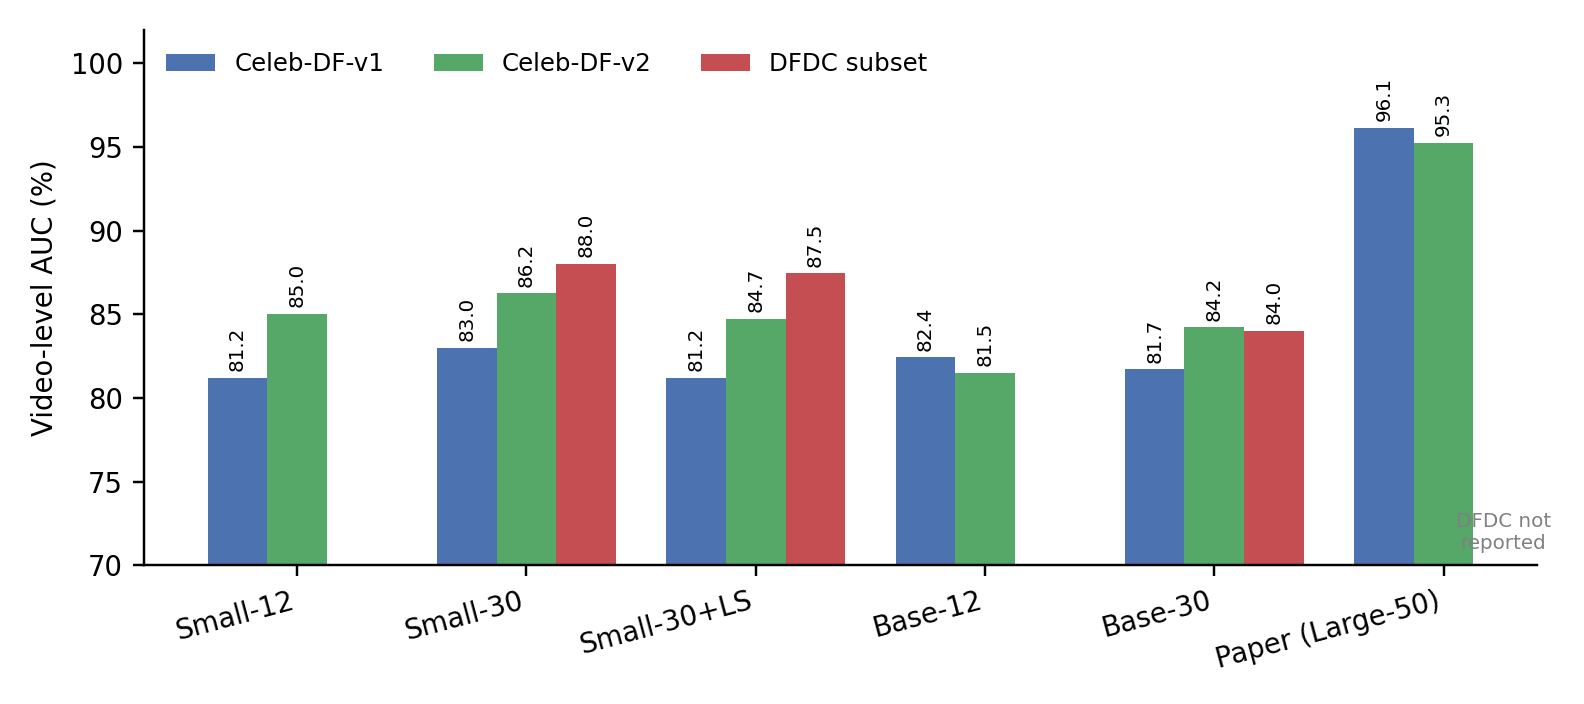
\includegraphics[width=0.78\textwidth]{fig_auc}
\caption{Cross-dataset video AUC of all configurations against the paper (n/r: not reported).}
\label{fig:auc}
\end{figure*}

\textbf{In-domain.} All our models reach 99.05--99.16\% FF++ validation AUC, within 0.4--0.5~pp of the paper's 99.56\%. Our FF++ EER is about 3.2--3.6\% versus the paper's 1.79\%; validation procedures may differ, so this comparison is indicative only.

\textbf{Cross-dataset.} Our best model (Small, 30 epochs) is 13.16~pp below the paper on Celeb-DF-v1 and 9.01~pp below on Celeb-DF-v2 (Fig.~\ref{fig:gap}). Reproducing high source-domain accuracy has therefore not reproduced the reported cross-dataset generalization.

\begin{figure}[!t]
\centering
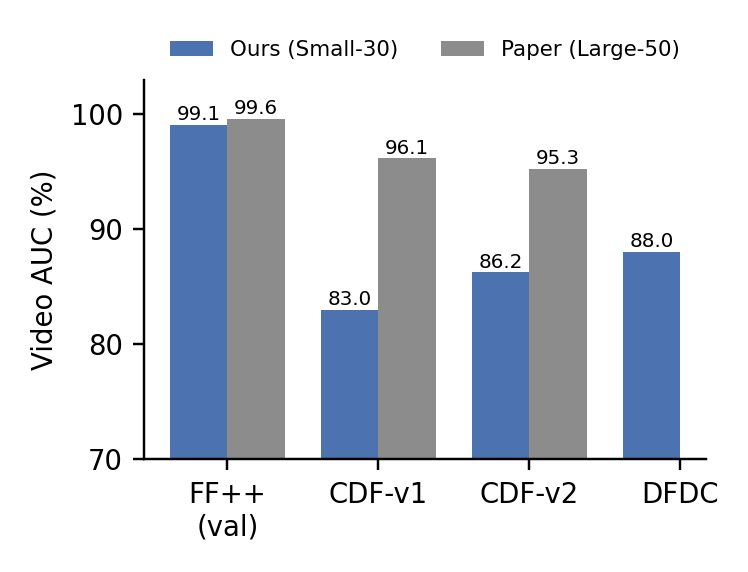
\includegraphics[width=2.9in]{fig_gap}
\caption{In-domain (FF++) versus unseen-dataset video AUC for Small, 30 epochs, and the paper.}
\label{fig:gap}
\end{figure}

\subsection{Equal Error Rate}
\begin{table}[!t]
\caption{Cross-dataset EER (\%), lower is better.\label{tab:eer}}
\centering
\footnotesize
\setlength{\tabcolsep}{3pt}
\begin{tabular}{|l|c||c|c|c|}
\hline
Model & Ep. & CDF-v1 & CDF-v2 & DFDC\\
\hline
Small & 12 & 30.65 & 22.94 & --\\
\textbf{Small} & \textbf{30} & \textbf{26.32} & \textbf{22.35} & \textbf{19.74}\\
Small + LS & 30 & 26.32 & 25.00 & 19.94\\
Base & 12 & 25.81 & 26.18 & --\\
Base & 30 & 28.95 & 23.82 & 23.68\\
\hline
Paper (Large) & 50 & n/r & 12.65 & n/r\\
\hline
\end{tabular}
\end{table}
Table~\ref{tab:eer} mirrors the AUC picture. Small at 30 epochs has the lowest EER on Celeb-DF-v2 (22.35\% versus 12.65\% for the paper) and on DFDC among the models evaluated there. On Celeb-DF-v1 the 12-epoch Base model has a slightly lower EER (25.81\%) than Small-30 (26.32\%) although its AUC is lower (82.43\% versus 82.98\%); AUC and EER summarise different parts of the ROC curve and need not agree.

\subsection{DFDC subset}
\begin{table}[!t]
\caption{DFDC subset (392 videos, 12{,}544 frames), \texttt{best.pt} checkpoints.\label{tab:dfdc}}
\centering
\footnotesize
\begin{tabular}{|l||c|c|c|}
\hline
Metric & Small & Base & Better\\
\hline
Video AUC (\%) & \textbf{88.03} & 84.00 & Small\\
EER (\%) & \textbf{19.74} & 23.68 & Small\\
Frame AUC (\%) & \textbf{79.99} & 78.10 & Small\\
\hline
\end{tabular}
\end{table}
Small is ahead on all three metrics (Table~\ref{tab:dfdc}): +4.03~pp video AUC, $-3.94$~pp EER. Video-level AUC exceeds frame-level AUC by 8.04~pp (Small) and 5.90~pp (Base), consistent with aggregation damping noisy single-frame predictions.

\textbf{Statistical uncertainty.} The subset is small and imbalanced (76 real, 316 fake). The Hanley--McNeil approximation~\cite{hanley1982meaning} gives a standard error of about 1.75~pp for an AUC of 88\%, i.e. a 95\% interval of roughly $\pm3.4$~pp. Small and Base are evaluated on the same videos, so their difference is paired and its uncertainty is smaller than for independent samples, but the 4.03~pp gap should still be treated as suggestive, not conclusive. Differences of 1--2~pp, which dominate the Celeb-DF comparisons (only 100 videos in v1), lie within sampling noise.

\section{Ablation Study}
All ablations change one factor relative to a stated reference; deltas are in pp.

\subsection{Training length (12 $\to$ 30 epochs)}
\begin{table}[!t]
\caption{Effect of 30 versus 12 epochs.\label{tab:epochs}}
\centering
\footnotesize
\setlength{\tabcolsep}{3pt}
\begin{tabular}{|l||c|c|c|c|}
\hline
Backbone & $\Delta$AUC v1 & $\Delta$EER v1 & $\Delta$AUC v2 & $\Delta$EER v2\\
\hline
Small & $+1.78$ & $-4.33$ & $+1.23$ & $-0.59$\\
Base & $-0.72$ & $+3.14$ & $+2.71$ & $-2.36$\\
\hline
\end{tabular}
\end{table}
Longer training helps Small on both Celeb-DF sets, but for Base the effect depends on the target dataset (Table~\ref{tab:epochs}). Training duration alone is not a reliable predictor of generalization. DFDC is not available for the 12-epoch models.

\subsection{Backbone size (Small versus Base)}
At 30 epochs, Base minus Small is $-1.27$~pp on Celeb-DF-v1, $-2.03$~pp on Celeb-DF-v2 and $-4.03$~pp on DFDC video AUC, even though Base has the higher FF++ validation AUC (99.16\% versus 99.08\%). A larger backbone did not translate into better cross-dataset performance here. At 12 epochs Base is $+1.23$~pp on v1 but $-3.51$~pp on v2.

\subsection{Label smoothing on the forgery-type loss}
\begin{table}[!t]
\caption{Small, 30 epochs: label smoothing 0.1 minus baseline.\label{tab:ls}}
\centering
\footnotesize
\begin{tabular}{|l||c|c|c|}
\hline
Dataset & $\Delta$ video AUC & $\Delta$ EER & $\Delta$ frame AUC\\
\hline
Celeb-DF-v1 & $-1.78$ & $0.00$ & n/a\\
Celeb-DF-v2 & $-1.51$ & $+2.65$ & n/a\\
DFDC subset & $-0.58$ & $+0.20$ & $+0.91$\\
\hline
\end{tabular}
\end{table}
The label-smoothed run (45{,}000 steps, best FF++ validation AUC 99.05\%) did not improve video AUC on any unseen set (Table~\ref{tab:ls}). DFDC frame-level AUC rose by 0.91~pp, so frame- and video-level results are not uniformly aligned. This is a single-seed result and does not show that label smoothing is generally ineffective. The baseline Celeb-DF numbers are final-checkpoint results whereas the label-smoothed evaluation used \texttt{best.pt}; this confound is disclosed in Section~\ref{sec:lim}.

\subsection{Auxiliary forgery-type supervision}
The paper's central claim is that the auxiliary type task helps authenticity detection. \todo{insert the no-auxiliary-loss run (dff\_noaux) results here if available; they are not in the status report}

\section{Discussion}
\textbf{Source-domain accuracy is not robustness.} With about 99\% FF++ validation AUC, Small-30 loses 16.10~pp on Celeb-DF-v1, 12.8~pp on Celeb-DF-v2 and 11.05~pp on DFDC. A detector can separate real from fake very well on data like its training set and still struggle when the source, manipulation pipeline, compression or identity distribution changes. Which factor dominates cannot be determined from these experiments, and the FF++ and DFDC numbers may not belong to the same checkpoint.

\textbf{Why the paper gap may exist.} Candidate causes are (i) the capacity and representation of DINOv2-Large versus Small/Base, (ii) the training recipe (50 epochs, learning rate $2\times10^{-4}$, weight decay $10^{-5}$ versus our $10^{-4}$ and 0.01), (iii) details of the adapter implementation, and (iv) differences in splits, cropping and aggregation. Because several differ at once, the comparison cannot attribute the gap to any one of them, and it does not by itself show that the paper is irreproducible or that our architecture is wrong.

\textbf{Bigger is not automatically better.} Base wins on FF++ but loses on DFDC on every metric. Plausible explanations (different learned representations, optimisation dynamics, interaction with the target data) remain hypotheses that need controlled runs.

\textbf{Longer training and overfitting.} The mixed effect of 12 versus 30 epochs is consistent with overfitting to the source dataset, but it does not establish it.

\textbf{Label smoothing.} We expected smoothed type labels to encourage features that are less specific to FF++ manipulations; the data do not support a benefit at $\epsilon=0.1$ in this run.

\section{Limitations}\label{sec:lim}
\begin{enumerate}
\item \textbf{Backbone mismatch.} The paper uses DINOv2-Large; we use Small and Base, so the comparison does not isolate implementation quality.
\item \textbf{Training mismatch.} Epochs, learning rate, weight decay, hardware and other details differ from the paper.
\item \textbf{Evaluation protocol.} Our manifests (100, 518 and 392 videos) have not been verified to match the paper's benchmark splits, and the DFDC subset is a subset, not the full dataset.
\item \textbf{Checkpoint inconsistency.} FF++ numbers are best-validation checkpoints, Celeb-DF numbers of baseline runs are final checkpoints, and DFDC and label-smoothing results use \texttt{best.pt}. The training durations behind each \texttt{best.pt} should be confirmed before treating Table~\ref{tab:auc} as a controlled comparison.
\item \textbf{Single seed.} No variance across seeds is available, so small differences cannot be separated from noise.
\item \textbf{No causal evidence.} The experiments show what changes, not why.
\item \textbf{Class imbalance and small $n$.} The DFDC subset has 76 real and 316 fake videos; Celeb-DF-v1 has only 100 videos. No confidence intervals beyond the approximation above were computed.
\item \textbf{No DFDC reference.} No DFDC score from the paper is available for comparison.
\end{enumerate}

\section{Conclusion and Future Work}
We reproduced DFF-Adapter on smaller DINOv2 backbones. In-domain FF++ validation AUC (99.08\%) is within 0.5~pp of the paper, but cross-dataset AUC on Celeb-DF is 9--13~pp lower, so the paper's generalization claims are not reproduced in our setting. Among our configurations, Small trained for 30 epochs is the strongest cross-dataset candidate (82.98\%, 86.25\%, 88.03\% on Celeb-DF-v1, Celeb-DF-v2 and DFDC). A larger backbone and label smoothing on the type loss did not help. The most defensible conclusion is that source-dataset performance alone is insufficient to judge a deepfake detector.

\textbf{Future work.} (1) Evaluate one selected checkpoint per model on all four datasets with a single scoring procedure. (2) Verify splits, cropping and aggregation against the paper's protocol. (3) Run at least three seeds for the best configuration. (4) Ablate adapter configuration, the auxiliary type loss and label smoothing one factor at a time. (5) Document how the DFDC subset was selected, and evaluate the 12-epoch models on DFDC. (6) Try DINOv2-Large and the paper's learning rate and weight decay if compute permits.

\bibliographystyle{IEEEtran}
\bibliography{ref}

{\appendix
\textbf{Platforms.} Training and evaluation ran as Kaggle notebooks on Tesla T4 GPUs (two GPUs used concurrently for two experiments); data were stored as private Kaggle datasets. Software: PyTorch, Hugging Face Transformers, safetensors, OpenCV, and MTCNN for face cropping. \todo{confirm library list and versions}

\textbf{Reliability measures.} The experiment runner was validated with a smoke test; unbuffered logging, periodic checkpoints (\texttt{last.pt}) and a time limit (\texttt{max\_hours}) were used so that long runs under Kaggle's commit mode could be monitored and recovered.

\textbf{Prompts and AI assistance.} AI assistants (ChatGPT and Claude) were used to review and debug the training and runner code, to design the smoke test, and to draft this report from our experiment notes; all numbers were taken from our saved experiment results. \todo{confirm and list prompts if required}
}

\end{document}
